\documentclass[conference]{IEEEtran}
\usepackage{array}
\usepackage[caption=true,font=footnotesize,labelfont=rm,textfont=rm]{subfig}
\usepackage{textcomp}
\usepackage{stfloats}
\usepackage{url}
\usepackage{verbatim}
\usepackage{graphicx}
\usepackage{tikz}
\usetikzlibrary{arrows.meta,positioning,fit,calc,backgrounds,shapes.geometric}
\hyphenation{op-tical net-works semi-conduc-tor IEEE-Xplore}
\def\BibTeX{{\rm B\kern-.05em{\sc i\kern-.025em b}\kern-.08em
    T\kern-.1667em\lower.7ex\hbox{E}\kern-.125emX}}
\usepackage{balance}

\usepackage{amssymb,amsfonts}
\usepackage[tbtags]{amsmath}

\usepackage[ruled,linesnumbered]{algorithm2e}
\usepackage{color}
\usepackage{booktabs}
\usepackage[thmmarks,amsmath]{ntheorem}
\usepackage{setspace}
\usepackage{hyperref}
\usepackage{cite}
\usepackage{soul}
\soulregister{\cite}7
\captionsetup{font={footnotesize}}
{
    \theoremstyle{nonumberplain}
    \theoremheaderfont{\bfseries\itshape}
    \theorembodyfont{\normalfont}
    \theoremseparator{:}
    \theoremsymbol{\ensuremath{\blacksquare}}
    \newtheorem{proof}{Proof}
}
{
    \theoremstyle{plain}
    \theoremheaderfont{\bfseries\itshape}
    \theorembodyfont{\normalfont}
    \theoremseparator{:}
    \theoremsymbol{\ensuremath{\blacksquare}}
    \newtheorem{remark}{Remark}
    \newtheorem{definition}{Definition}
    \newtheorem{lemma}{Lemma}
    \newtheorem{theorem}{Theorem}
}

\newcommand{\algref}[1]{\textit{\textbf{Algorithm \ref{#1}}}}
\newcommand{\theoref}[1]{\textit{\textbf{Theorem \ref{#1}}}}
\newcommand{\lemmref}[1]{\textit{\textbf{Lemma \ref{#1}}}}
\newcommand{\defref}[1]{\textit{\textbf{Definition \ref{#1}}}}
\newcommand{\figref}[1]{Fig. \ref{#1}}
\providecommand{\resultfigdir}{figures}
\providecommand{\methodfigdir}{figures}
\pdfoutput=1

\begin{document}

\title{DiffFNO: Structured Diffusion Policy with Fourier Neural Operators for IoT-Enabled Multi-Zone HVAC Control}

\author{Wei Zou, Yu Sun, Haibo Zhou,~\IEEEmembership{Fellow,~IEEE}}

\maketitle

\begin{abstract}
IoT sensor networks enable real-time thermal monitoring and control command delivery, making data-driven HVAC optimization promising for building energy management. However, multi-zone HVAC control remains difficult for standard reinforcement learning policies because actions are coupled across zones, unimodal policies are restrictive, and MLP backbones do not explicitly model zone-wise coordination. This paper presents DiffFNO, a generative controller for IoT-enabled multi-zone HVAC systems. It combines a conditional diffusion policy with an FNO denoiser acting on the action-dimension axis and a residual pathway that preserves local corrective flexibility. Experiments on the BEAR OfficeSmall-Hot\_Dry benchmark show that DiffFNO improves the overall energy--comfort trade-off over Diffusion-MLP while producing smoother and more physically consistent control signals. Compared with its no-residual counterpart, DiffFNO incurs slightly higher energy consumption but substantially fewer comfort violations, indicating that the residual branch helps the controller make finer adjustments near comfort boundaries.
\end{abstract}

\begin{IEEEkeywords}
IoT-enabled buildings, HVAC control, diffusion policy, Fourier neural operator, reinforcement learning.
\end{IEEEkeywords}

\section{Introduction}

Buildings account for a substantial portion of global energy consumption, and HVAC systems are among the largest controllable contributors to operational energy use \cite{perez2008review,cao2016building,cuce2026role}. In IoT-enabled buildings, distributed sensors continuously monitor zone temperatures, outdoor conditions, solar irradiance, and occupancy-related loads. These measurements are aggregated through gateway nodes and fed into the control policy at each decision step. The resulting control actions are then applied to zone-level HVAC actuators through the same IoT infrastructure, closing the sensing--actuation loop. This closed-loop digital infrastructure makes data-driven HVAC control increasingly relevant for large commercial buildings.

Recent RL approaches provide a model-free alternative to rule-based control and model predictive control (MPC), but standard policies remain mismatched to multi-zone HVAC control in three ways \cite{drgovna2020all,wei2017deep,biemann2021experimental,mason2019review,alsayed2024hvacreview}. First, many continuous-control methods use deterministic mappings or unimodal Gaussian action distributions, which are too restrictive when multiple coordinated control patterns are feasible under the same thermal state. Second, common multilayer perceptron (MLP) backbones do not explicitly encode cross-zone coupling and therefore struggle to capture the structured geometry of the joint action vector. Third, unguided policies often generate oscillatory actions, which may increase energy use, reduce comfort, and weaken physical consistency in coupled building systems.

Diffusion policies offer a more expressive action model for continuous control \cite{chi2025diffusion,janner2022planning,wang2023diffusion}, while Fourier Neural Operators (FNOs) provide a useful spectral prior when dominant low-frequency coordination is desired \cite{li2021fourier,qin2024toward,liu2024mitigating}. Motivated by these observations, we formulate the multi-zone HVAC policy as a conditional reverse-diffusion process and replace the standard MLP denoiser with an FNO backbone that acts directly on the action-dimension axis. We further retain a residual pathway so the denoiser can preserve coarse spectral coordination while still making local corrective adjustments when comfort boundaries are tight. Intuitively, the action-dimension axis can be viewed as a compact control field over thermal zones: neighboring or strongly coupled zones should usually receive coordinated commands, while abrupt high-frequency variations across action coordinates often indicate physically inconsistent control. This makes an FNO-based spectral prior well aligned with multi-zone HVAC actions. The same perspective is also aligned with networked building automation, where decisions are made from synchronized multi-zone measurements rather than isolated room observations. The policy class should therefore be able to represent multiple feasible joint actions, preserve cross-zone consistency, and remain stable under repeated sensor-driven updates.

This formulation differs from two nearby lines of work. Unlike conventional building RL, the policy is not treated as a point estimator over each action coordinate; instead, the full multi-zone command is modeled as a generated object. Unlike generic diffusion control, building-specific structure is introduced through spectral action modeling and residual local correction. This combination tailors DiffFNO to centralized IoT-enabled HVAC control rather than a direct application of a generic diffusion policy. In particular, once IoT sensing aggregates building-wide measurements into a common state vector, the controller must map that shared state to a coordinated joint action, which directly motivates a state-conditional generative policy with explicit action-space structure.

The main contributions of this work are:
\begin{itemize}
    \item We propose \emph{DiffFNO}, an IoT-oriented generative HVAC controller that models the full joint zone action through conditional diffusion rather than point-estimate regression.
    \item We introduce an FNO denoiser over the action-dimension axis together with a residual local-correction pathway, enabling coordinated low-frequency control without losing the ability to react near comfort boundaries.
    \item We show on the BEAR benchmark that DiffFNO improves the energy--comfort profile over Diffusion-MLP, and that removing the residual branch yields lower energy and smoother actions only at the cost of increased comfort violations.
\end{itemize}

The remainder of this paper is organized as follows. Section~\ref{sec:system_model} introduces the multi-zone HVAC control model. Section~\ref{sec:method} presents the proposed DiffFNO framework. Section~\ref{sec:experiments} reports the experimental setup and results. Finally, Section~\ref{sec:conclusion} concludes the paper and discusses future extensions.

\section{System Model}
\label{sec:system_model}

\begin{figure}[!t]
    \captionsetup{width=\linewidth}
    \IfFileExists{figures/Control Architecture.pdf}{
        \centerline{\includegraphics[width=\linewidth]{figures/Control Architecture.pdf}}
    }{
        \centering
        \resizebox{0.98\linewidth}{!}{
        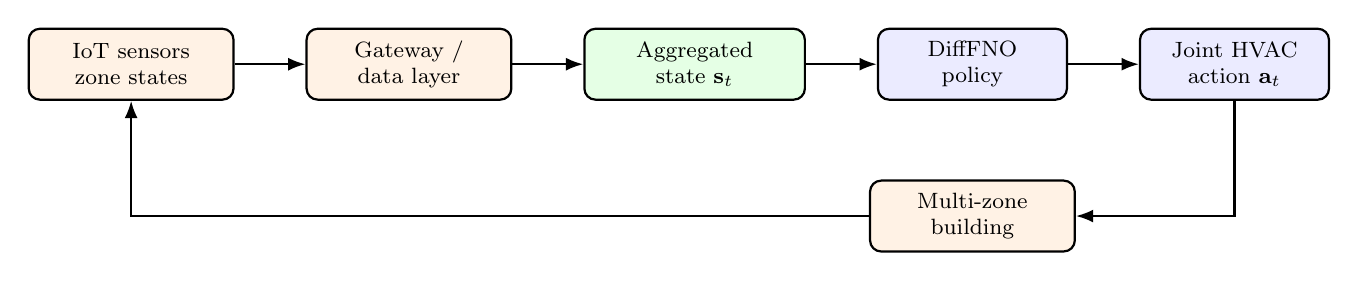
\begin{tikzpicture}[
            font=\footnotesize,
            node distance=7mm and 8mm,
            block/.style={draw, rounded corners, thick, align=center, minimum height=9mm, minimum width=24mm, fill=blue!8},
            state/.style={draw, rounded corners, thick, align=center, minimum height=9mm, minimum width=28mm, fill=green!10},
            data/.style={draw, rounded corners, thick, align=center, minimum height=9mm, minimum width=26mm, fill=orange!10},
            arrow/.style={-{Latex[length=2.2mm]}, thick}
        ]
            \node[data] (sensor) {IoT sensors\\zone states};
            \node[data, right=9mm of sensor] (gateway) {Gateway /\\data layer};
            \node[state, right=9mm of gateway] (statev) {Aggregated\\state $\mathbf{s}_t$};
            \node[block, right=9mm of statev] (policy) {DiffFNO\\policy};
            \node[block, right=9mm of policy] (act) {Joint HVAC\\action $\mathbf{a}_t$};
            \node[data, below=10mm of policy] (building) {Multi-zone\\building};

            \draw[arrow] (sensor) -- (gateway);
            \draw[arrow] (gateway) -- (statev);
            \draw[arrow] (statev) -- (policy);
            \draw[arrow] (policy) -- (act);
            \draw[arrow] (act.south) |- (building.east);
            \draw[arrow] (building.west) -| (sensor.south);
        \end{tikzpicture}}
    }
    \caption{IoT-enabled sensing--control architecture for multi-zone building HVAC control. Zone-level measurements are gathered by the gateway node, aggregated into the state vector $\mathbf{s}_t$, and fed to the control policy, whose joint action is applied back to the building.}
    \label{fig:system_model}
\end{figure}

Figure~\ref{fig:system_model} illustrates the closed-loop IoT architecture considered in this work. Zone-level sensing data are gathered through the gateway node, stored and retrieved through the building data layer, and aggregated into the state vector $\mathbf{s}_t$ used by the policy. The resulting joint control action is then applied back to the zone-level HVAC actuators. We formulate multi-zone HVAC control as a discounted MDP $\mathcal{M}=(\mathcal{S},\mathcal{A},\mathcal{P},r,\gamma)$, where the transition kernel is induced by the physics-based BEAR simulator \cite{zhang2023bear}. The controller interacts with a six-zone office building under coupled thermal dynamics, weather disturbances, solar gains, and internal loads. The state vector $\mathbf{s}_t$ is constructed from aggregated IoT measurements collected across all thermal zones, including zone temperatures, outdoor temperature, solar irradiance, ground temperature, and internal loads. In Fig.~\ref{fig:system_model}, the retrieved-data block highlights the main components of $\mathbf{s}_t$, while the ellipsis denotes additional exogenous features such as the ground-temperature term. The action is a continuous joint HVAC command for all $N$ zones:
\begin{equation}
    \mathbf{a}_t =
    [a_{t,1}, a_{t,2}, \dots, a_{t,N}]
    \in [-1,1]^N,
    \label{eq:action}
\end{equation}
so the policy must generate a coordinated multi-zone control vector rather than independent per-zone decisions. Because the six zones share disturbances and thermal interactions, a command that appears locally beneficial for one zone may still be globally inefficient once neighboring temperatures, comfort violations, and total HVAC energy are considered jointly.

The reward combines the simulator reward with an explicit thermal-comfort violation penalty:
\begin{equation}
    d_{t,i}=\left|T_{t,i}^{\mathrm{zone}}-T^{\mathrm{ref}}\right|,
    \qquad
    V_t=\sum_{i=1}^{N}\mathbb{I}(d_{t,i}>\delta),
    \label{eq:violation}
\end{equation}
\begin{equation}
    r_t = \rho \left( r_t^{\mathrm{env}} - \lambda V_t \right),
    \label{eq:reward}
\end{equation}
where $T^{\mathrm{ref}}$ is the target temperature, $\delta$ is the comfort tolerance, $V_t$ counts zone-wise temperature violations with respect to the comfort band defined by ASHRAE Standard 55 \cite{standard2023thermal}, $\lambda$ is the violation penalty, and $\rho$ is a reward-scaling coefficient. The control objective is
\begin{equation}
    J(\pi)=\mathbb{E}_{\pi}\left[\sum_{t=0}^{T-1}\gamma^t r_t\right].
    \label{eq:objective}
\end{equation}
This objective matches the control target of reducing HVAC energy while avoiding persistent comfort-band violations across the monitored thermal zones.

\section{DiffFNO Method}
\label{sec:method}

\subsection{Conditional Diffusion Policy}

Instead of regressing a single action from $\mathbf{s}_t$, we generate actions through a conditional denoising process \cite{ho2020denoising}. Let $\mathbf{x}_0$ denote the clean action and $\mathbf{x}_k$ its noisy version at reverse step $k$. Under the variance-preserving parameterization,
\begin{equation}
    \mathbf{x}_k =
    \sqrt{\bar{\alpha}_k}\mathbf{x}_0 +
    \sqrt{1-\bar{\alpha}_k}\boldsymbol{\epsilon},
    \qquad
    \boldsymbol{\epsilon}\sim\mathcal{N}(\mathbf{0},\mathbf{I}),
    \label{eq:noisy_action}
\end{equation}
and the denoiser directly predicts the clean action
\begin{equation}
    \hat{\mathbf{x}}_0 = f_{\theta}(\mathbf{x}_k, k, \mathbf{s}_t).
    \label{eq:x0_prediction}
\end{equation}
Under the standard DDPM parameterization, the reverse posterior mean can be written as
\begin{equation}
    \boldsymbol{\mu}_k(\hat{\mathbf{x}}_0,\mathbf{x}_k)=
    c_1(k)\hat{\mathbf{x}}_0 + c_2(k)\mathbf{x}_k,
    \label{eq:posterior_mean}
\end{equation}
where $c_1(k)$ and $c_2(k)$ are determined by the noise schedule. Starting from Gaussian noise, the policy iteratively reconstructs a feasible multi-zone action through reverse DDPM sampling. This formulation is attractive for HVAC control because it can represent richer action distributions than deterministic or unimodal Gaussian policies while exposing the structure of the joint action to the denoiser.

\begin{figure*}[!t]
    \centering
    \IfFileExists{figures/DiffFNO framework for IoT-enabled multi-zone HVAC control.pdf}{
        \includegraphics[width=\textwidth]{figures/DiffFNO framework for IoT-enabled multi-zone HVAC control.pdf}
    }{
        \resizebox{\textwidth}{!}{
        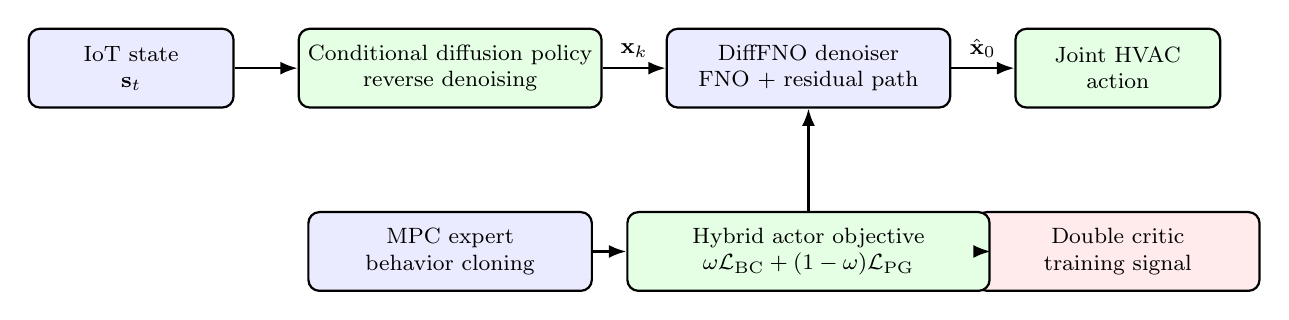
\begin{tikzpicture}[
            font=\footnotesize,
            node distance=6mm and 8mm,
            box/.style={draw, rounded corners, thick, align=center, minimum height=10mm, minimum width=28mm, fill=blue!8},
            mid/.style={draw, rounded corners, thick, align=center, minimum height=10mm, minimum width=24mm, fill=green!10},
            crit/.style={draw, rounded corners, thick, align=center, minimum height=10mm, minimum width=24mm, fill=red!8},
            arrow/.style={-{Latex[length=2.2mm]}, thick}
        ]
            \node[box, minimum width=26mm] (state) {IoT state\\$\mathbf{s}_t$};
            \node[mid, right=8mm of state, minimum width=36mm] (diff) {Conditional diffusion policy\\reverse denoising};
            \node[box, right=8mm of diff, minimum width=36mm] (fno) {DiffFNO denoiser\\FNO + residual path};
            \node[mid, right=8mm of fno, minimum width=26mm] (action) {Joint HVAC\\action};

            \draw[arrow] (state) -- (diff);
            \draw[arrow] (diff) -- node[above] {$\mathbf{x}_k$} (fno);
            \draw[arrow] (fno) -- node[above] {$\hat{\mathbf{x}}_0$} (action);

            \node[box, below=13mm of diff, minimum width=36mm] (expert) {MPC expert\\behavior cloning};
            \node[crit, below=13mm of action, minimum width=36mm] (qtrain) {Double critic\\training signal};
            \node[mid, below=13mm of fno, minimum width=46mm] (train) {Hybrid actor objective\\$\omega \mathcal{L}_{\mathrm{BC}} + (1-\omega)\mathcal{L}_{\mathrm{PG}}$};
            \draw[arrow] (expert) -- (train);
            \draw[arrow] (qtrain) -- (train);
            \draw[arrow] (train) -- (fno);
        \end{tikzpicture}}
    }
    \caption{DiffFNO framework. The policy models the joint action through reverse diffusion, the DiffFNO denoiser imposes spectral structure on the action-dimension axis, and the residual pathway preserves local corrective flexibility. A double critic is used during training, while deployment uses unguided reverse sampling.}
    \label{fig:difffno_framework}
\end{figure*}

\subsection{DiffFNO Backbone}

The main limitation of an MLP denoiser is that it treats the action vector as an unordered coordinate array. In contrast, multi-zone HVAC control requires the action to be generated as a coordinated control field across thermal zones. We therefore replace the MLP backbone with an FNO denoiser that operates directly along the action-dimension axis. Given noisy action $\mathbf{x}_k$, diffusion step $k$, and state $\mathbf{s}_t$, the latent feature map is updated by
\begin{equation}
    \mathbf{Y}^{(\ell+1)} =
    \sigma\!\left(
    \mathcal{K}_{\mathrm{spec}}^{(\ell)}(\mathbf{Y}^{(\ell)}) +
    \mathcal{K}_{\mathrm{pw}}^{(\ell)}(\mathbf{Y}^{(\ell)}) +
    \mathbf{h}_c
    \right),
    \label{eq:spectral_layer}
\end{equation}
where $\mathcal{K}_{\mathrm{spec}}^{(\ell)}$ is a truncated one-dimensional spectral convolution, $\mathcal{K}_{\mathrm{pw}}^{(\ell)}$ is a pointwise convolution, and $\mathbf{h}_c$ is the joint embedding of state and diffusion-step information. The final clean-action estimate is
\begin{equation}
    f_{\theta}(\mathbf{x}_k,k,\mathbf{s}_t)=
    \hat{\mathbf{y}}_k + \mathrm{sigmoid}(g)\mathbf{W}_r\mathbf{x}_k.
    \label{eq:final_denoiser}
\end{equation}
Here $\hat{\mathbf{y}}_k$ is the spectrally structured output of the FNO trunk and the gated residual term re-injects local coordinate information from the noisy action. This design encourages globally coordinated low-frequency action patterns while retaining enough local flexibility for zone-specific comfort regulation. In the present conference version, this residual pathway is an essential part of the main method because it improves comfort compliance relative to the no-residual alternative.

\subsection{Hybrid Training Framework}

Although deployment uses unguided reverse diffusion, the actor is still trained within an off-policy actor--critic framework. We use a conservative double critic
\begin{equation}
    Q_{\phi}^{\min}(\mathbf{s},\mathbf{a})=
    \min\{Q_{\phi_1}(\mathbf{s},\mathbf{a}),Q_{\phi_2}(\mathbf{s},\mathbf{a})\},
    \label{eq:qmin}
\end{equation}
for policy evaluation during training. The actor combines diffusion-consistent behavior cloning from MPC demonstrations with critic-driven policy improvement:
\begin{equation}
    \mathcal{L}_{\mathrm{BC}}=
    \mathbb{E}\left[
    \left\|
    f_{\theta}(\mathbf{x}_k^{\mathrm{exp}},k,\mathbf{s}_t)-
    \mathbf{a}_t^{\mathrm{exp}}
    \right\|_2^2
    \right],
    \label{eq:bc_loss}
\end{equation}
\begin{equation}
    \mathcal{L}_{\mathrm{PG}}=
    -\mathbb{E}_{\mathbf{s}_t}\left[
    Q_{\phi}^{\min}(\mathbf{s}_t,\pi_{\theta}(\mathbf{s}_t))
    \right],
    \label{eq:pg_loss}
\end{equation}
\begin{equation}
    \mathcal{L}_{\mathrm{actor}}=
    \omega \mathcal{L}_{\mathrm{BC}}+
    (1-\omega)\mathcal{L}_{\mathrm{PG}},
    \label{eq:actor_loss}
\end{equation}
where $\mathcal{L}_{\mathrm{BC}}$ reconstructs expert actions from noisy inputs and $\mathcal{L}_{\mathrm{PG}}$ maximizes the conservative critic value \cite{fujimoto2021minimalist}. A high initial $\omega$ stabilizes early learning, and the weight is then decayed so that the policy can move beyond imitation while preserving physically meaningful action priors. This hybrid design allows the actor to inherit low-jitter control behavior from MPC before refining the policy with long-horizon value information. At deployment time, however, the controller executes the learned DiffFNO policy without any additional critic-based inference correction.

\section{Experiments}
\label{sec:experiments}

\subsection{Setup}

We evaluate all methods on the BEAR OfficeSmall-Hot\_Dry benchmark \cite{zhang2023bear}, which models a six-zone office building under Tucson hot-dry weather. The controller receives synchronized sensor-style state streams at each control step and returns zone-wise HVAC commands through the same interface. The control interval is one hour and each episode lasts $168$ steps. Unless otherwise stated, all methods share the same target temperature, comfort band, simulator disturbances, and reward setting, which helps isolate controller quality rather than task-definition changes. We compare DiffFNO against DiffFNO w/o Residual, Diffusion-MLP, MPC, SAC, and SAC+MPC. The two unguided diffusion variants share the same training pipeline and differ only in whether the residual branch is enabled, while Diffusion-MLP replaces the spectral denoiser with a standard MLP backbone. Expert demonstrations are generated by MPC with planning horizon $3$. Learning-based methods report three-seed statistics to reflect training variability. We report four complementary metrics: episode HVAC energy, comfort violations, final test reward, and mean absolute action change. Energy and violations reflect the primary building objective, final reward reflects the optimized RL objective, and mean absolute action change captures temporal smoothness of the generated control sequence.

\begin{table}[t]
\centering
\caption{Shared hyperparameters for the learning-based methods.}
\label{tab:training_setup}
\scriptsize
\setlength{\tabcolsep}{3.5pt}
\renewcommand{\arraystretch}{1.04}
\begin{tabular}{>{\raggedright\arraybackslash}p{0.29\linewidth}>{\raggedright\arraybackslash}p{0.18\linewidth}>{\raggedright\arraybackslash}p{0.29\linewidth}>{\raggedright\arraybackslash}p{0.18\linewidth}}
\toprule
Setting & Value & Setting & Value \\
\midrule
Training steps & $1.0\times 10^6$ & Batch size / replay buffer & $256$ / $10^6$ \\
Discount / $n$-step return & $0.99$ / $3$ & Update-per-step & $0.5$ \\
Actor / critic learning rate & $10^{-4}$ / $2\times 10^{-5}$ & Diffusion steps $K$ & $6$ \\
FNO width / retained modes & $48$ / $4$ & Spectral layers / activation & $1$ / Mish \\
Residual branch & enabled & BC weight schedule $\omega$ & $0.8 \rightarrow 0.1$ \\
\bottomrule
\end{tabular}
\end{table}

\textbf{Inference cost.} DiffFNO uses only $K=6$ reverse diffusion steps at deployment. Because inference does not require critic-gradient correction, the online cost is dominated by a short denoising chain and remains small relative to the one-hour control interval used in BEAR.

\begin{table*}[!t]
\centering
\caption{Overall comparison on the BEAR OfficeSmall-Hot\_Dry task. Learning-based methods report the three-seed mean $\pm$ standard deviation. Lower mean $|\Delta a|$ indicates smoother control.}
\label{tab:overall_results}
\footnotesize
\setlength{\tabcolsep}{4.5pt}
\renewcommand{\arraystretch}{1.10}
\begin{tabular}{lcccc}
\hline
Method & Energy (kWh) $\downarrow$ & Violations $\downarrow$ & Test Reward $\uparrow$ & Mean $|\Delta a|$ $\downarrow$ \\
\hline
DiffFNO & 901.3 $\pm$ 19.9 & \textbf{0.886 $\pm$ 0.135} & \textbf{-0.738 $\pm$ 0.086} & 0.0402 $\pm$ 0.0090 \\
DiffFNO w/o Residual & \textbf{871.1 $\pm$ 6.6} & 1.082 $\pm$ 0.338 & -0.844 $\pm$ 0.207 & 0.0357 $\pm$ 0.0109 \\
Diffusion-MLP & 990.9 $\pm$ 38.4 & 1.441 $\pm$ 0.510 & -1.106 $\pm$ 0.321 & 0.0596 $\pm$ 0.0162 \\
MPC & 1004.9 & 1.780 & -1.325 & \textbf{0.0130} \\
SAC & 5980.4 $\pm$ 27.3 & 5.483 $\pm$ 0.046 & -5.055 $\pm$ 0.011 & 0.3430 $\pm$ 0.0412 \\
SAC+MPC & 1864.6 $\pm$ 74.6 & 3.431 $\pm$ 0.294 & -2.600 $\pm$ 0.222 & 0.1729 $\pm$ 0.0117 \\
\hline
\end{tabular}
\end{table*}

\subsection{Overall Performance}

Table~\ref{tab:overall_results} shows that DiffFNO achieves the most favorable comfort--reward balance within the unguided diffusion family. Although DiffFNO w/o Residual obtains lower raw energy and slightly smoother actions, the main model reduces comfort violations from $1.082$ to $0.886$ and improves the final test reward from $-0.844$ to $-0.738$. This pattern suggests that the residual branch trades a modest amount of efficiency for more effective corrective behavior near comfort boundaries.

\begin{figure}[!t]
    \centering
    
\includegraphics[width=\linewidth]{\resultfigdir/compare_energy_violations_noguide_main.pdf}
    \caption{Energy--comfort Pareto comparison for the conference method set. Points show three-seed means and error bars show one standard deviation. The diffusion points include DiffFNO, DiffFNO w/o Residual, and Diffusion-MLP.}
    \label{fig:energy_violations}
\end{figure}

The Pareto view in Fig.~\ref{fig:energy_violations} reinforces the same conclusion. DiffFNO and DiffFNO w/o Residual form the local Pareto frontier among the learned diffusion variants: the no-residual model is more energy efficient, whereas DiffFNO occupies the lower-violation operating point. In contrast, Diffusion-MLP is both less efficient and less comfort-compliant, while SAC-based baselines remain far from the relevant operating regime for this benchmark. It is also worth clarifying the role of MPC in this comparison. Although MPC provides the expert demonstrations used for behavior cloning, the expert itself is generated with a short planning horizon of $3$ steps. After initialization from these demonstrations, the learned policy can improve beyond the expert by optimizing the full long-horizon return under the shared reward while retaining the stabilizing prior induced by expert imitation. Two comparisons are especially informative here: the gap between DiffFNO and Diffusion-MLP shows that expressive diffusion alone is not sufficient, whereas the gap between DiffFNO and DiffFNO w/o Residual shows that lower energy and smoother actuation can still come at the cost of more comfort violations.

\subsection{Action Quality and Ablation}

The spectral prior imposed by DiffFNO is reflected in the physical HVAC signal. As shown in Fig.~\ref{fig:physical_psd_compare}, DiffFNO concentrates substantially more spectrum mass in the low-frequency region than Diffusion-MLP and moves closer to the smooth operating pattern of MPC. Using the $2$ cycles/day cutoff in the Welch spectrum, DiffFNO assigns $82.6\%$ of HVAC power spectral mass to the low-frequency region, compared with $95.2\%$ for physical MPC and $73.7\%$ for Diffusion-MLP. The result is consistent with the lower mean $|\Delta a|$ values in Table~\ref{tab:overall_results}: the proposed controller improves the overall control objective while generating a signal with more physically regular temporal structure than the MLP-denoiser baseline.

\begin{figure}[!t]
    \centering
    
\includegraphics[width=\linewidth]{\resultfigdir/smalloffice_physical_psd_compare_noguide_main.pdf}
    \caption{HVAC power spectral density comparison for physical MPC, DiffFNO, and Diffusion-MLP; the learned-controller curves are averaged over three seeds. The dashed line marks the $2$ cycles/day cutoff.}
    \label{fig:physical_psd_compare}
\end{figure}

The ablation summary in Fig.~\ref{fig:ablation_heatmap} clarifies the role of each module within the conference narrative. Replacing the MLP denoiser with DiffFNO improves comfort, smoothness, and terminal performance. Removing the residual branch yields lower energy and smoother action increments, but it also reduces comfort compliance, which is consistent with the interpretation that the residual pathway restores useful local flexibility near comfort boundaries. In Fig.~\ref{fig:ablation_heatmap}, the ``Convergence'' column is computed from the normalized terminal evaluation reward across ablation variants, so it should be read as a compact terminal-performance indicator rather than as a claim about the full dynamic convergence trajectory. From a control perspective, building HVAC decisions are repeatedly executed over long horizons, and a policy that reduces energy but produces unstable or high-frequency commands may still be undesirable under coupled thermal dynamics. The smoother low-frequency behavior of DiffFNO therefore matters not only as a diagnostic statistic but also as evidence that the learned controller is better aligned with the physical regularity of building operation.

Taken together, the experiments suggest a clear division of labor among the model components. Diffusion provides expressive joint-action generation, DiffFNO injects a structural prior for coordinated multi-zone control, and the residual branch improves comfort-oriented local correction. This decomposition matches the empirical pattern in Table~\ref{tab:overall_results} and Fig.~\ref{fig:ablation_heatmap}, where no single simplified variant preserves all three advantages at once. The proposed design does not rely on handcrafted rules tied to a specific room or actuator. Instead, it relies on a generic centralized interface: a vector of sensor-derived building states, a vector of zone-wise control commands, and a reward that trades energy against comfort compliance. As long as that interface is available, the same modeling principle can be applied to other multi-zone buildings, climates, or supervisory control layers, although the final quantitative gains should still be validated case by case. The present results are based on the BEAR OfficeSmall-Hot\_Dry task with hourly control, so they identify DiffFNO as an effective policy class for this representative setting rather than as a universal solution across all building configurations.

\begin{figure}[!t]
    \centering
    
\includegraphics[width=\linewidth]{\resultfigdir/ablation_summary_heatmap_noguide_main.pdf}
    \caption{Normalized ablation summary across energy, comfort, smoothness, and convergence for the unguided conference variants. Each column is min--max normalized over DiffFNO, DiffFNO w/o Residual, and Diffusion-MLP.}
    \label{fig:ablation_heatmap}
\end{figure}

\section{Conclusion}
\label{sec:conclusion}

This paper presents DiffFNO for IoT-enabled multi-zone building HVAC control. By combining conditional diffusion, an FNO denoiser over the joint action vector, and a residual local-correction pathway, the method produces smoother and more coordinated control actions while improving the energy--comfort trade-off over the MLP-denoiser baseline on BEAR OfficeSmall-Hot\_Dry.

The results suggest a simple design principle for building control: when the action itself has meaningful physical structure, the policy class should encode that structure explicitly, but it should also preserve enough local flexibility to respond near comfort boundaries. Future work will extend this conference version toward a journal study that incorporates inference-time critic guidance on top of DiffFNO, analyzes how guidance interacts with the residual pathway, and validates the expanded framework across additional building types, climates, and safety-aware settings.

\balance
\bibliographystyle{IEEEtran}
\bibliography{references}

\end{document}
